\documentclass[11pt]{article}
\usepackage[margin=1in]{geometry}
\usepackage[T1]{fontenc}
\usepackage{lmodern,microtype,amsmath,amssymb,amsthm}
\usepackage{tikz}
\usepackage[hidelinks]{hyperref}
\setlength{\parindent}{0pt}
\setlength{\parskip}{0.6em}
\newcommand{\C}{\mathbb C}
\newcommand{\R}{\mathbb R}
\newcommand{\ww}{\mathbf w}
\newcommand{\hh}{\mathbf h}
\DeclareMathOperator{\Real}{Re}
\DeclareMathOperator{\Imag}{Im}
\newtheorem*{theorem}{Theorem}
\title{MATH 411 --- Lecture 4}
\author{}
\date{September 12 (date on the handwritten notes)}
\begin{document}
\maketitle
\vspace{-2em}
\textit{Transcribed from all seven handwritten pages, retaining the order and
intermediate calculations. Abbreviations have been expanded. A correction to
the real-analysis criterion is explicitly noted below; supplementary details
completing arguments only stated in the handwriting are identified as such.}

% Handwritten page 1.
\section{Complex differentiability and total differentiability}
Let $f:U\to\C$, where $U\subseteq\C$ is open. The function $f$ is
\emph{complex differentiable at $w\in U$} if
\[
 \lim_{h\to0}\frac{f(w+h)-f(w)}{h}
\]
exists. This limit is denoted by $f'(w)$.

Alternatively, there exist a function $\sigma$ defined in a small
neighbourhood of $0\in\C$ and a complex number $\xi\in\C$ such that
\begin{enumerate}
\item $f(w+h)-f(w)-\xi h=\sigma(h)h$;
\item $\displaystyle\lim_{h\to0}\sigma(h)=0$.
\end{enumerate}
The neighbourhood is chosen small enough that $w+h\in U$. The small sketch
in the notes indicates that $\sigma$ is defined around the origin.
In this formulation $\xi=f'(w)$.

Now let $F$ be a function on an open set $U\subseteq\R^2$, with
\[
 F:U\to\R^2,\qquad
 \begin{pmatrix}x\\y\end{pmatrix}\longmapsto
 \begin{pmatrix}u(x,y)\\v(x,y)\end{pmatrix}.
\]
The function $F$ is said to be \emph{totally differentiable} at the point
$\ww=\begin{pmatrix}x\\y\end{pmatrix}$ if there exists a real matrix
$D_{\ww}$ such that
\[
 \lim_{\|\hh\|\to0}
 \frac{F(\ww+\hh)-F(\ww)-D_{\ww}\hh}{\|\hh\|}
 =\begin{pmatrix}0\\0\end{pmatrix}.
\]
Here $\hh$ is a vector in $\R^2$, and $\|\hh\|$ is its Euclidean norm.

% Handwritten page 2.
\subsection*{Criterion from real analysis}
If the first partial derivatives of $u$ and $v$ exist in a neighbourhood
of $\ww$ and are continuous at $\ww$, then $F$ is totally differentiable
at $\ww$, and its derivative matrix is the Jacobian
\[
 D_{\ww}=J_F(\ww)=
 \begin{pmatrix}u_x&u_y\\v_x&v_y\end{pmatrix}_{\ww}.
\]
\textit{Correction to the handwriting:} the notes put an
``if and only if'' between total differentiability and the existence and
continuity of the partial derivatives. Continuity of the partial derivatives
is a sufficient condition, but it is not a necessary condition for total
differentiability at a point.

\section{The relation between the two notions of differentiability}
What is the relation between total differentiability of $F$ and complex
differentiability of $f$? Write
\[
 f:U\to\C,\qquad f(x+iy)=u(x,y)+iv(x,y),\qquad
 F(x,y)=\begin{pmatrix}u(x,y)\\v(x,y)\end{pmatrix}.
\]
The naive guess is
\[
 F\text{ is totally differentiable at }\ww
 \quad\Longleftrightarrow\quad
 f\text{ is complex differentiable at }w.
\]
This guess is false. The correct statement is the following.
\begin{theorem}
The function $f$ is complex differentiable at $w=x+iy$ if and only if
$F=\begin{pmatrix}u\\v\end{pmatrix}$ is totally differentiable at
$\ww=\begin{pmatrix}x\\y\end{pmatrix}$ and
\[
 \boxed{u_x=v_y,\qquad u_y=-v_x}
\]
at $(x,y)$. These are the \emph{Cauchy--Riemann equations}.
\end{theorem}

\subsection*{Notation: holomorphic and entire functions}
If $f:U\to\C$ is complex differentiable at every point $w\in U$, we say
that $f$ is \emph{holomorphic on $U$}. We write
\[
 \mathcal H(U)=\{\text{all holomorphic functions on }U\}.
\]
% Handwritten page 3.
A function in $\mathcal H(\C)$, that is, a function holomorphic at every
$z\in\C$, is called \emph{entire}.

\section{Proof of the theorem: the forward implication}
Suppose $f$ is complex differentiable at $w=x+iy$, and write
$f(x+iy)=u(x,y)+iv(x,y)$. We want to show that
\[
 F(x,y)=\begin{pmatrix}u(x,y)\\v(x,y)\end{pmatrix}
\]
is totally differentiable and that the Cauchy--Riemann equations hold.

\subsection{Why is the associated real function totally differentiable?}
Since $f$ is complex differentiable, there exist a function $\sigma$ on
a neighbourhood of $0$ and a number $\alpha\in\C$ such that
\[
 f(w+h)-f(w)-\alpha h=\sigma(h)h,
 \qquad \lim_{h\to0}\sigma(h)=0.
\]
Set
\[
 \ww=\begin{pmatrix}x\\y\end{pmatrix},\qquad
 \hh=\begin{pmatrix}r\\s\end{pmatrix},\qquad h=r+is.
\]
Then
\[
 F(\ww+\hh)-F(\ww)=
 \begin{pmatrix}
 u(x+r,y+s)-u(x,y)\\
 v(x+r,y+s)-v(x,y)
 \end{pmatrix}.
\]
We seek a matrix $D_{\ww}$ for which the components of
$F(\ww+\hh)-F(\ww)-D_{\ww}\hh$ are the real and imaginary parts of
\[
 f(w+h)-f(w)-\alpha h=\sigma(h)h.
\]
% Handwritten page 4.
Write $\alpha=a+ib$. Since $h=r+is$, we have
\begin{align*}
 \alpha h&=(a+ib)(r+is)\\
 &=ar+ias+ibr+i^2bs\\
 &=(ar-bs)+i(as+br).
\end{align*}
The corresponding real matrix multiplication is
\[
 \begin{pmatrix}a&-b\\b&a\end{pmatrix}
 \begin{pmatrix}r\\s\end{pmatrix}
 =\begin{pmatrix}ar-bs\\as+br\end{pmatrix}.
\]
Therefore choose
\[
 D_{\ww}=\begin{pmatrix}a&-b\\b&a\end{pmatrix}.
\]
By what we have just observed,
\[
 F(\ww+\hh)-F(\ww)-D_{\ww}\hh
 =\begin{pmatrix}\Real(\sigma(h)h)\\\Imag(\sigma(h)h)\end{pmatrix}.
\]
By assumption, $\lim_{h\to0}\sigma(h)=0$. What, then, is
\[
 \lim_{h\to0}\frac{\sigma(h)h}{|h|}?
\]
For $h\ne0$, write $h=|h|e^{i\theta_h}$. Thus
\[
 \frac{\sigma(h)h}{|h|}=\sigma(h)e^{i\theta_h}.
\]
The number $e^{i\theta_h}$ lies on the unit circle. Consequently,
\[
 \left|\frac{\sigma(h)h}{|h|}\right|
 =|\sigma(h)|\,|e^{i\theta_h}|=|\sigma(h)|\longrightarrow0,
\]
and hence
\[
 \lim_{h\to0}\frac{\sigma(h)h}{|h|}=0.
\]
If this complex expression tends to zero, its real and imaginary parts
also tend to zero:
\[
 \Real\left(\frac{\sigma(h)h}{|h|}\right)\longrightarrow0,
 \qquad
 \Imag\left(\frac{\sigma(h)h}{|h|}\right)\longrightarrow0.
\]
But $\|\hh\|=\sqrt{r^2+s^2}=|h|$, so
\[
 \begin{pmatrix}
 \Real\left(\dfrac{\sigma(h)h}{|h|}\right)\\[0.7em]
 \Imag\left(\dfrac{\sigma(h)h}{|h|}\right)
 \end{pmatrix}
 =\frac{F(\ww+\hh)-F(\ww)-D_{\ww}\hh}{\|\hh\|}.
\]
Both components tend to zero. This is exactly the definition of total
differentiability of $F$ at $\ww$.

% Handwritten page 5.
\subsection{Why do the Cauchy--Riemann equations hold?}
We now verify that the components $u$ and $v$ of the associated real
function satisfy the Cauchy--Riemann equations. Write $z=x+iy$ and
\[
 f(z)=u(x,y)+iv(x,y).
\]
\begin{center}
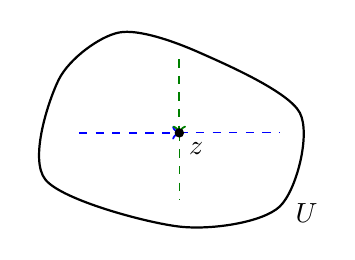
\begin{tikzpicture}[scale=0.85]
 \draw[thick] plot[smooth cycle] coordinates
 {(-2,-0.7) (-1.8,0.8) (-0.9,1.5) (0.3,1.2) (1.8,0.3) (1.5,-1.1) (0,-1.4)};
 \draw[blue,dashed,->,thick] (-1.5,0)--(0,0);
 \draw[blue,dashed] (0,0)--(1.5,0);
 \draw[green!50!black,dashed,->,thick] (0,1.1)--(0,0);
 \draw[green!50!black,dashed] (0,0)--(0,-1);
 \fill (0,0) circle (2pt);
 \node[below right] at (0,0) {$z$};
 \node at (1.9,-1.2) {$U$};
\end{tikzpicture}
\end{center}
First approach horizontally, so the complex increment is $h+i0$ with
$h\in\R$. Then
\begin{align*}
 f'(z)
 &=\lim_{\substack{h\to0\\h\in\R}}\frac{f(z+h)-f(z)}{h}\\
 &=\lim_{\substack{h\to0\\h\in\R}}
 \frac{u(x+h,y)+iv(x+h,y)-u(x,y)-iv(x,y)}{h}\\
 &=\lim_{\substack{h\to0\\h\in\R}}
 \frac{u(x+h,y)-u(x,y)}{h}
 +i\lim_{\substack{h\to0\\h\in\R}}
 \frac{v(x+h,y)-v(x,y)}{h}\\
 &=u_x(x,y)+iv_x(x,y).
\end{align*}
Thus
\[
 \boxed{f'(z)=u_x+iv_x.}
\]
Next approach along the vertical axis. The complex increment is now $ih$,
where $h\in\R$. By the definition of the complex derivative, using this
vertical approach gives the same limit:
\[
 f'(z)=\lim_{\substack{h\to0\\h\in\R}}
 \frac{f(z+ih)-f(z)}{ih}.
\]
% Handwritten page 6.
Expanding this expression yields
\begin{align*}
 f'(z)
 &=\lim_{\substack{h\to0\\h\in\R}}
 \frac{u(x,y+h)+iv(x,y+h)-u(x,y)-iv(x,y)}{ih}\\
 &=\lim_{\substack{h\to0\\h\in\R}}
 \frac{u(x,y+h)-u(x,y)}{ih}
 +\lim_{\substack{h\to0\\h\in\R}}
 \frac{i\bigl(v(x,y+h)-v(x,y)\bigr)}{ih}\\
 &=\frac1i\lim_{\substack{h\to0\\h\in\R}}
 \frac{u(x,y+h)-u(x,y)}{h}
 +\lim_{\substack{h\to0\\h\in\R}}
 \frac{v(x,y+h)-v(x,y)}{h}\\
 &=-iu_y(x,y)+v_y(x,y),\qquad\text{since }\frac1i=-i.
\end{align*}
Therefore
\[
 \boxed{f'(z)=-iu_y+v_y=u_x+iv_x.}
\]
Equating real and imaginary parts gives
\[
 \boxed{u_x=v_y,\qquad v_x=-u_y.}
\]
This proves the forward implication: complex differentiability of $f$
implies total differentiability of $F$ and the Cauchy--Riemann equations.
The handwritten notes now use the theorem as established. In particular,
existence and continuity of the first partial derivatives, together with
the Cauchy--Riemann equations, imply complex differentiability.

\subsection*{Supplementary completion: the reverse implication}
\textit{The handwriting does not work out this direction. It is included
here to complete the stated equivalence without leaving steps implicit.}
Suppose $F$ is totally differentiable at $\ww$ and the Cauchy--Riemann
equations hold there. Its derivative matrix is
\[
 D_{\ww}=\begin{pmatrix}u_x&u_y\\v_x&v_y\end{pmatrix}
 =\begin{pmatrix}a&-b\\b&a\end{pmatrix},
 \qquad a=u_x=v_y,\quad b=v_x=-u_y.
\]
Set $\alpha=a+ib$ and let
\[
 E(\hh)=F(\ww+\hh)-F(\ww)-D_{\ww}\hh
 =\begin{pmatrix}E_1(\hh)\\E_2(\hh)\end{pmatrix}.
\]
Total differentiability means $\|E(\hh)\|/\|\hh\|\to0$.
For $h=r+is$ corresponding to $\hh=(r,s)^{\mathsf T}$, the matrix
calculation above gives
\[
 f(w+h)-f(w)-\alpha h=E_1(\hh)+iE_2(\hh).
\]
For $h\ne0$, divide by $h$ and take absolute values:
\begin{align*}
 \left|\frac{f(w+h)-f(w)}h-\alpha\right|
 &=\frac{|E_1(\hh)+iE_2(\hh)|}{|h|}\\
 &=\frac{\sqrt{E_1(\hh)^2+E_2(\hh)^2}}{\|\hh\|}\\
 &=\frac{\|E(\hh)\|}{\|\hh\|}\longrightarrow0.
\end{align*}
Thus $f'(w)$ exists and equals $\alpha=u_x+iv_x$.

\section{Examples}
\subsection{The exponential function is entire}
Let $z=x+iy$. Use the theorem to prove that $e^z$ is entire. We must
verify that the first partial derivatives exist and are continuous, and
that $u$ and $v$ satisfy the Cauchy--Riemann equations.
\begin{align*}
 e^z&=e^x e^{iy}\\
 &=e^x\bigl(\cos y+i\sin y\bigr)\\
 &=\underbrace{e^x\cos y}_{u(x,y)}
   +i\underbrace{e^x\sin y}_{v(x,y)}.
\end{align*}
The four partial derivatives are
\begin{align*}
 u_x&=e^x\cos y,&v_x&=e^x\sin y,\\
 u_y&=-e^x\sin y,&v_y&=e^x\cos y.
\end{align*}
They exist and are continuous everywhere, and
\[
 u_x=v_y,\qquad u_y=-v_x.
\]
The derivative matrix has precisely the indicated pattern:
\[
 J_F=\begin{pmatrix}
 e^x\cos y&-e^x\sin y\\
 e^x\sin y&e^x\cos y
 \end{pmatrix}.
\]
Hence the theorem shows that $e^z$ is entire. The derivative formula also gives
\[
 (e^z)'=u_x+iv_x=e^x\cos y+ie^x\sin y=e^z.
\]

% Handwritten page 7.
\subsection{The Cauchy--Riemann equations alone do not suffice}
Just because $u$ and $v$ satisfy the Cauchy--Riemann equations does not
mean that $f(z)=u(x,y)+iv(x,y)$ is complex differentiable. For example, let
\[
 f(z)=\begin{cases}
 \dfrac{z^5}{|z|^4},&z\ne0,\\[0.6em]
 0,&z=0.
 \end{cases}
\]
This function satisfies the Cauchy--Riemann equations at the origin but
is not complex differentiable there.

\textit{Supplementary verification of the partial derivatives asserted
in the notes.} For real $t\ne0$, $|t|^4=t^4$ and $i^5=i$, so
\[
 f(t)=\frac{t^5}{|t|^4}=t,\qquad
 f(it)=\frac{i^5t^5}{|it|^4}=it.
\]
Thus $u(t,0)=t$, $v(t,0)=0$, $u(0,t)=0$, $v(0,t)=t$, and
$u(0,0)=v(0,0)=0$. Consequently,
\begin{align*}
 u_x(0,0)&=\lim_{t\to0}\frac{u(t,0)-u(0,0)}t
 =\lim_{t\to0}\frac tt=1,\\
 v_x(0,0)&=\lim_{t\to0}\frac{v(t,0)-v(0,0)}t
 =\lim_{t\to0}\frac0t=0,\\
 u_y(0,0)&=\lim_{t\to0}\frac{u(0,t)-u(0,0)}t
 =\lim_{t\to0}\frac0t=0,\\
 v_y(0,0)&=\lim_{t\to0}\frac{v(0,t)-v(0,0)}t
 =\lim_{t\to0}\frac tt=1.
\end{align*}
Hence $u_x(0,0)=v_y(0,0)$ and $u_y(0,0)=-v_x(0,0)$.

The handwritten difference-quotient calculation is
\begin{align*}
 \lim_{h\to0}\frac{f(0+h)-f(0)}h
 &=\lim_{h\to0}\frac{f(h)}h\\
 &=\lim_{h\to0}\frac{h^5/|h|^4}{h}\\
 &=\lim_{h\to0}\frac{h^4}{|h|^4},
\end{align*}
which does not exist. To make that last assertion explicit, write
$h=re^{i\theta}$, where $r>0$. Then
\[
 \frac{h^4}{|h|^4}=\frac{r^4e^{4i\theta}}{r^4}=e^{4i\theta}.
\]
Along the positive real axis ($\theta=0$), this quotient equals $1$.
Along the ray $\theta=\pi/4$, it equals $e^{i\pi}=-1$.
Both paths approach the origin as $r\to0$, but give different limits.
Therefore $f'(0)$ does not exist.

\subsection{Polar form of the Cauchy--Riemann equations}
Suppose $f$ is written in polar coordinates, with $z=re^{i\theta}$ and $r>0$:
\[
 f(r,\theta)=u(r,\theta)+iv(r,\theta).
\]
The Cauchy--Riemann equations take the form stated in the notes:
\[
 \boxed{u_r=\frac1r v_\theta,\qquad
 \frac1r u_\theta=-v_r.}
\]
\textit{Supplementary derivation of the displayed formula.}
Since $x=r\cos\theta$ and $y=r\sin\theta$, the chain rule gives
\begin{align*}
 u_r&=u_x\cos\theta+u_y\sin\theta,\\
 v_r&=v_x\cos\theta+v_y\sin\theta,\\
 u_\theta&=-r u_x\sin\theta+r u_y\cos\theta,\\
 v_\theta&=-r v_x\sin\theta+r v_y\cos\theta.
\end{align*}
Substituting $v_x=-u_y$ and $v_y=u_x$ yields
\begin{align*}
 \frac1r v_\theta
 &=-v_x\sin\theta+v_y\cos\theta\\
 &=u_y\sin\theta+u_x\cos\theta=u_r,\\[0.3em]
 \frac1r u_\theta
 &=-u_x\sin\theta+u_y\cos\theta\\
 &=-v_y\sin\theta-v_x\cos\theta=-v_r.
\end{align*}
\end{document}
